% SPDX-License-Identifier: CC-BY-4.0
\documentclass{article}
\usepackage[margin=1in]{geometry}
\usepackage{graphicx} 
\usepackage[colorlinks=true, urlcolor=blue, linkcolor=red]{hyperref}

\begin{document}
\author{David Meeker}
\title{Sintered NdFeB Magnet Properties}
\maketitle

The N30-N55 properties defined in FEMM are meant to be representative of typical examples rather than strictly based on the products from one vendor.  The properties were generated using information from \url{https://en.wikipedia.org/wiki/Neodymium_magnet}. This Wikipedia page defines the following properties:

\begin{itemize}
\item Relative Permeability (\(\mu_r\)) = 1.05
\item Electrical Resistivity =  110–170 $\mu \Omega$·cm
\end{itemize}

An electrical resistivity of 150 $\mu \Omega$·cm was selected as a reasonable median value in a fairly broad range.  The corresponding electrical conductivity required by FEMM is $\sigma$ = 0.667~MS/m.

On the basis of data from many vendors, the numerical designation of the magnet grade represents the best-case energy product in units of MGOe as measured at room temperature (20°C) for a range of energy product usually spanning a range of 2~MGOe.  However, magnets are rarely delivered magnetized to this best-case magnetization.  For this reason, it is assumed that the actual energy product is the numerical grade minus one in units of MGOe, \textit{i.e.} an N42 magnet has an energy product of 41MGOe at 20°C.

Defining \(BH_{max}\) as the energy product of the magnet and assuming a straight-line demagnetization curve, the magnet's normal coercivity, \(H_{cB}\) is defined by:
\[H_{cB} = 2 \sqrt{\frac{BH_{max}}{\mu_r \mu_o}} \]
where \(\mu_o\) represents the magnetic permeability of free space.  Then, the remanent magnetization, \(B_r\) is defined as:
\[B_r = \mu_r \mu_o H_{cB}\]
For grades N48 and higher, there is a noticeable knee in the second-quadrant demagnetization curve.  For N48, N50, N52, and N55, the location of the knee was selected on the basis of examining various manufacturer's specs. The resulting demagnetization curves are shown below in Figure 1.

\begin{figure}
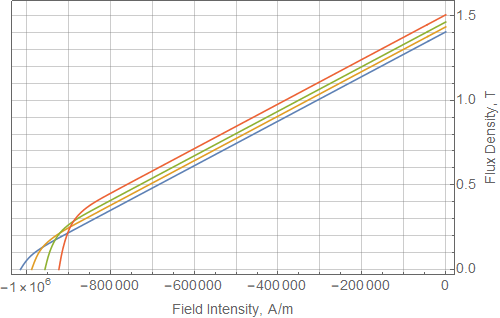
\includegraphics{mystrongmagnets.png}
\caption{Assumed demagnetization curves of N48, N50, N52, and N55}
\end{figure}

The result list of NdFeB grades and representative material properties is summarized below in Table 1.

\begin{table}
\centering
\begin{tabular} {|c|c|c|c|c|c|c|}
\hline
Grade & \(BH_{max}\), MGOe & \(B_r\), T & \(B_r\), kG & \(H_{cB}\), kA/m & \(H_{cB}\), kOe & \(\sigma\), MS/m \\ \hline \hline
N30 & 29 & 1.104 & 11.04 & 836 & 10.51 & 0.667 \\ \hline
N33 & 32 & 1.159 & 11.59 & 879 & 11.04 & 0.667 \\ \hline
N35 & 34 & 1.195 & 11.95 & 906 & 11.38 & 0.667 \\ \hline
N38 & 37 & 1.247 & 12.47 & 945 & 11.87 & 0.667 \\ \hline
N40 & 39 & 1.280 & 12.80 & 970 & 12.19 & 0.667 \\ \hline
N42 & 41 & 1.312 & 13.12 & 995 & 12.50 & 0.667 \\ \hline
N45 & 44 & 1.359 & 13.59 & 1030 & 12.95 & 0.667 \\ \hline
N48 & 47 & 1.405 & 14.05 & 1015 & 12.75 & 0.667 \\ \hline
N50 & 49 & 1.435 & 14.35 & 988 & 12.41 & 0.667 \\ \hline
N52 & 51 & 1.464 & 14.64 & 956 & 12.02 & 0.667 \\ \hline
N55 & 54 & 1.506 & 15.06 & 923 & 11.60 & 0.667 \\ \hline
\end{tabular}
\caption{Representative NdFeB Material Grades at 20°C.}
\end{table}

\subsection*{References}

\noindent Arnold Magnetic Technologies, \href{https://web.archive.org/web/20200513225014/https://www.arnoldmagnetics.com/wp-content/uploads/2019/06/Arnold-Neo-Catalog.pdf}{Neodynium Iron Boron Magnet Catalog}, accessed 13 May 2020.

\noindent Dexter Magnetic Technologies, \href{https://web.archive.org/web/20220123232850/https://www.dextermag.com/wp-content/uploads/2016/10/Dexter_Nd-Fe-B__Curves_Properties_Table.pdf}{Dexter Catalog}, accessed 23 Jan 2022.

\noindent Electron Energy Corporation \href{https://web.archive.org/web/20251010021738/https://www.electronenergy.com/hubfs/EEC_NdFeB_Information.pdf}{Neodymium Iron Boron Magnets}, accessed 10 Oct 2025.

\noindent Copyright 2026 David Meeker. This document is licensed under the \href{https://creativecommons.org/licenses/by/4.0/}{Creative Commons Attribution 4.0 International License (CC BY 4.0)}.

\end{document}